\documentclass[8pt,aspectratio=169]{beamer}
\usetheme{Madrid}
\usepackage{graphicx}
\usepackage{booktabs}
\usepackage{adjustbox}
\usepackage{multicol}
\usepackage{amsmath}

% Color definitions
\definecolor{mlblue}{RGB}{0,102,204}
\definecolor{mlpurple}{RGB}{51,51,178}
\definecolor{mllavender}{RGB}{173,173,224}
\definecolor{mllavender2}{RGB}{193,193,232}
\definecolor{mllavender3}{RGB}{204,204,235}
\definecolor{mllavender4}{RGB}{214,214,239}
\definecolor{mlorange}{RGB}{255, 127, 14}
\definecolor{mlgreen}{RGB}{44, 160, 44}
\definecolor{mlred}{RGB}{214, 39, 40}
\definecolor{mlgray}{RGB}{127, 127, 127}
\definecolor{lightgray}{RGB}{240, 240, 240}
\definecolor{midgray}{RGB}{180, 180, 180}

% Theme colors
\setbeamercolor{palette primary}{bg=mllavender3,fg=mlpurple}
\setbeamercolor{palette secondary}{bg=mllavender2,fg=mlpurple}
\setbeamercolor{palette tertiary}{bg=mllavender,fg=white}
\setbeamercolor{palette quaternary}{bg=mlpurple,fg=white}
\setbeamercolor{structure}{fg=mlpurple}
\setbeamercolor{section in toc}{fg=mlpurple}
\setbeamercolor{subsection in toc}{fg=mlblue}
\setbeamercolor{title}{fg=mlpurple}
\setbeamercolor{frametitle}{fg=mlpurple,bg=mllavender3}
\setbeamercolor{block title}{bg=mllavender2,fg=mlpurple}
\setbeamercolor{block body}{bg=mllavender4,fg=black}

\setbeamertemplate{navigation symbols}{}
\setbeamertemplate{itemize items}[circle]
\setbeamertemplate{enumerate items}[default]
\setbeamersize{text margin left=5mm,text margin right=5mm}

\newcommand{\bottomnote}[1]{%
\vfill
\vspace{-2mm}
\textcolor{mllavender2}{\rule{\textwidth}{0.4pt}}
\vspace{1mm}
\footnotesize
\textbf{#1}
}

% === Additional packages for mini-lecture ===
\usepackage{tikz}
\usepackage{pgfplots}
\pgfplotsset{compat=1.18}
\usetikzlibrary{arrows.meta, positioning, shapes.geometric, decorations.pathreplacing}

% === Mini-lecture accent colors (skill-documented values) ===
\definecolor{dfteal}{RGB}{0, 153, 153}
\definecolor{dfred}{RGB}{204, 51, 51}

% === Exampleblock styling ===
\setbeamercolor{exampleblock title}{bg=dfteal!20,fg=dfteal!80!black}
\setbeamercolor{exampleblock body}{bg=dfteal!5,fg=black}

% === Compact list command (MUST be defined before any usage) ===
\newcommand{\compactlist}{\setlength{\itemsep}{1pt}\setlength{\parskip}{0pt}\setlength{\parsep}{0pt}}

\title{Platform and Token Economics in Digital Finance}
\subtitle{Businesses that produce nothing are worth more than those that produce everything---why?}
\author{Economics of Digital Finance}
\institute{BSc Course}
\date{}

\begin{document}
\begin{frame}[plain]
\titlepage
\end{frame}

% ============================================================
% SLIDE 1: WHY -- Why is a company that makes nothing worth more?
% Visual: TikZ comic (dfteal dilemma) RIGHT, text LEFT
% ============================================================
\begin{frame}[t]{Why is a company that makes nothing worth more than one that makes everything?}
\begin{columns}[T]
\begin{column}{0.55\textwidth}
\small
A bakery makes bread. A factory makes cars. But the most valuable companies
in the world often make\ldots{} nothing at all. They simply connect people who
want to trade, share rides, or exchange messages. These are platforms
(businesses that create value by connecting two or more groups of users rather
than producing goods themselves). How can connecting people be worth more than
making things?

\vspace{2mm}
\footnotesize
\begin{itemize}\compactlist
\item Traditional businesses create value by producing goods or services
\item Platforms create value by facilitating interactions between groups
\item The more users a platform has, the more valuable it becomes to each user
\item This self-reinforcing growth explains why platforms dominate modern markets
\end{itemize}
\end{column}
\begin{column}{0.42\textwidth}
\centering
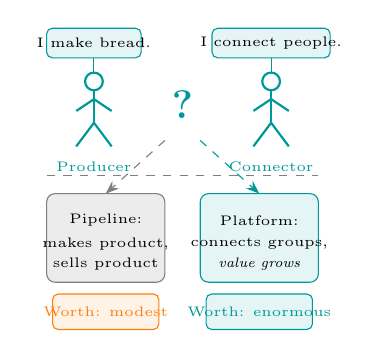
\begin{tikzpicture}[scale=0.75, every node/.style={font=\tiny}]
  % Producer stick figure (LEFT)
  \draw[dfteal, thick] (0.8,6.2) circle (0.15);
  \draw[dfteal, thick] (0.8,6.05) -- (0.8,5.5);
  \draw[dfteal, thick] (0.8,5.9) -- (0.5,5.7);
  \draw[dfteal, thick] (0.8,5.9) -- (1.1,5.7);
  \draw[dfteal, thick] (0.8,5.5) -- (0.5,5.1);
  \draw[dfteal, thick] (0.8,5.5) -- (1.1,5.1);
  \node[below, dfteal] at (0.8,5.0) {Producer};

  % Producer speech bubble
  \draw[dfteal, rounded corners=2pt, fill=dfteal!10]
    (0.0,6.6) rectangle (1.6,7.1);
  \node at (0.8,6.85) {I make bread.};
  \draw[dfteal] (0.8,6.6) -- (0.8,6.35);

  % Connector stick figure (RIGHT)
  \draw[dfteal, thick] (3.8,6.2) circle (0.15);
  \draw[dfteal, thick] (3.8,6.05) -- (3.8,5.5);
  \draw[dfteal, thick] (3.8,5.9) -- (3.5,5.7);
  \draw[dfteal, thick] (3.8,5.9) -- (4.1,5.7);
  \draw[dfteal, thick] (3.8,5.5) -- (3.5,5.1);
  \draw[dfteal, thick] (3.8,5.5) -- (4.1,5.1);
  \node[below, dfteal] at (3.8,5.0) {Connector};

  % Connector speech bubble
  \draw[dfteal, rounded corners=2pt, fill=dfteal!10]
    (2.8,6.6) rectangle (4.8,7.1);
  \node at (3.8,6.85) {I connect people.};
  \draw[dfteal] (3.8,6.6) -- (3.8,6.35);

  % Central question mark
  \node[font=\Large\bfseries, dfteal] at (2.3,5.8) {?};

  % Dividing line
  \draw[mlgray, dashed] (0,4.6) -- (4.6,4.6);

  % LEFT box: Pipeline outcome
  \draw[mlgray, rounded corners=3pt, fill=mlgray!15]
    (0.0,2.8) rectangle (2.0,4.3);
  \node[align=center] at (1.0,3.85) {Pipeline:};
  \node[align=center] at (1.0,3.45) {makes product,};
  \node[align=center] at (1.0,3.1) {sells product};
  % Value label -- Critic note 1: qualitative labels, not dollar amounts
  \draw[mlorange, rounded corners=2pt, fill=mlorange!10]
    (0.1,2.0) rectangle (1.9,2.6);
  \node[mlorange] at (1.0,2.3) {Worth: modest};

  % RIGHT box: Platform outcome
  \draw[dfteal, rounded corners=3pt, fill=dfteal!10]
    (2.6,2.8) rectangle (4.6,4.3);
  \node[align=center] at (3.6,3.85) {Platform:};
  \node[align=center] at (3.6,3.45) {connects groups,};
  \node[align=center, font=\tiny\itshape] at (3.6,3.1) {value grows};
  % Value label -- Critic note 1: qualitative labels, not dollar amounts
  \draw[dfteal, rounded corners=2pt, fill=dfteal!10]
    (2.7,2.0) rectangle (4.5,2.6);
  \node[dfteal] at (3.6,2.3) {Worth: enormous};

  % Dashed arrows from question mark to boxes
  \draw[dashed, ->, >=Stealth, mlgray] (2.0,5.2) -- (1.0,4.3);
  \draw[dashed, ->, >=Stealth, dfteal] (2.6,5.2) -- (3.6,4.3);
\end{tikzpicture}
\end{column}
\end{columns}

\begin{block}{Key Insight}
Platforms grow in value with each additional user, while traditional businesses must build
a new factory for each new customer---this is why connectors outvalue producers.
\end{block}

\bottomnote{Platform economics (the study of how businesses that connect user groups create and capture value) explains why the most valuable companies make nothing at all.}
\end{frame}

% ============================================================
% SLIDE 2: FEEL -- How many platforms did you use today?
% Visual: Full-width text-only with exampleblock
% ============================================================
\begin{frame}[t]{How many platforms did you use today without even thinking about it?}
\small
This morning, you woke up and checked your messages on one platform. You ordered
a ride on another. You paid for coffee through a third. You scrolled through
content curated by a fourth. Each of these services works because two groups
need each other: riders need drivers, buyers need sellers, viewers need creators.
Without both sides, the platform is worthless.

\vspace{3mm}
\footnotesize
\textit{Count the platforms you used before arriving at this lecture. For each one,
identify the two groups the platform connects. How many could you easily replace
with a competitor?}

\vspace{3mm}
\footnotesize
The difficulty of that last question reveals something important. When all your
contacts use one messaging app, or all merchants accept one payment network,
switching becomes costly even if a better alternative exists. This is lock-in
(when switching costs trap users on a platform even when better alternatives
exist), and it is one of the most powerful forces in platform economics. The
same dynamics that make platforms useful also make them hard to leave.

\begin{exampleblock}{Reflection}
Every platform you use today exists because it solved a coordination problem: it convinced
both sides to show up at the same time. The question is whether you chose it---or whether
you are trapped.
\end{exampleblock}

\bottomnote{Two-sided markets (platforms connecting two user groups who need each other) are the foundation of digital finance---from payment networks to decentralized exchanges.}
\end{frame}

% ============================================================
% SLIDE 3: WHAT -- What makes a platform different?
% Visual: Comparison table LEFT, text RIGHT
% ============================================================
\begin{frame}[t]{What makes a platform different from a regular business?}
\begin{columns}[T]
\begin{column}{0.55\textwidth}
\small
A pipeline business (one that creates value by producing and selling goods
in a linear chain) makes something and sells it: raw materials in, finished
product out. A platform business creates value differently: it connects two
or more groups and lets them transact with each other. The platform itself
produces nothing---it orchestrates interactions.

\vspace{1mm}
\begin{adjustbox}{max width=\linewidth}
\scriptsize
\begin{tabular}{lll}
\toprule
\textbf{Dimension} & \textbf{Pipeline (Bakery)} & \textbf{Platform (Exchange)} \\
\midrule
\shortstack[l]{Value\\creation} & \shortstack[l]{Produces goods\\or services} & \shortstack[l]{Connects groups\\who need each other} \\[2pt]
\shortstack[l]{Key\\asset} & \shortstack[l]{Factories,\\inventory} & \shortstack[l]{User base,\\network data} \\[2pt]
\shortstack[l]{Growth\\driver} & \shortstack[l]{More production\\capacity} & \shortstack[l]{More users attract\\more users} \\[2pt]
Competition & \shortstack[l]{Price and\\quality} & \shortstack[l]{Network size\\and lock-in} \\[2pt]
\shortstack[l]{Revenue\\model} & \shortstack[l]{Markup on\\cost of goods} & \shortstack[l]{Transaction fees\\or subscriptions} \\[2pt]
\shortstack[l]{Failure\\mode} & \shortstack[l]{Costs exceed\\revenue} & \shortstack[l]{Users leave---value\\collapses for all} \\
\bottomrule
\end{tabular}
\end{adjustbox}
\end{column}
\begin{column}{0.42\textwidth}
\footnotesize
The critical difference: a pipeline's value scales with production capacity.
A platform's value scales with users---and it scales faster. Each new user
makes the platform more valuable for every existing user. Economists call
this a network effect (when a product becomes more valuable as more people
use it).

\vspace{2mm}
\footnotesize
The failure mode is equally different. A pipeline can lose customers gradually.
A platform can collapse suddenly: once users start leaving, the network effect
reverses, and each departure makes the platform less valuable for those who
remain. This is a network effect in reverse---a death spiral.
\end{column}
\end{columns}

\begin{block}{Key Insight}
A platform's greatest strength---network effects that multiply value with each new
user---is also its greatest vulnerability: the same feedback loop can accelerate collapse
just as quickly as it accelerated growth.
\end{block}

\bottomnote{Network effects (when a product becomes more valuable as more people use it) are the engine of platform dominance---and the trigger of platform collapse.}
\end{frame}

% ============================================================
% SLIDE 4: CASE -- Follow one token from launch to dominance or death
% Visual: TikZ step diagram LEFT, narration RIGHT
% ============================================================
\begin{frame}[t]{Follow one token from launch to either dominance or death}
\begin{columns}[T]
\begin{column}{0.55\textwidth}
\centering
% Note: 0.85 scale -- step diagram, not comic
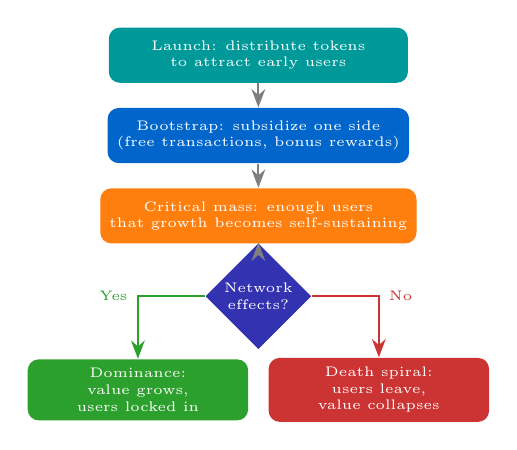
\begin{tikzpicture}[scale=0.85, every node/.style={font=\tiny},
  box/.style={rounded corners=4pt, minimum width=3.8cm, minimum height=0.7cm,
              align=center, text=white, font=\tiny}]
  % Box 1: Launch
  \node[box, fill=dfteal] (b1) at (0,6.0)
    {Launch: distribute tokens\\to attract early users};
  % Box 2: Bootstrap
  \node[box, fill=mlblue] (b2) at (0,4.8)
    {Bootstrap: subsidize one side\\(free transactions, bonus rewards)};
  % Box 3: Critical mass
  \node[box, fill=mlorange] (b3) at (0,3.6)
    {Critical mass: enough users\\that growth becomes self-sustaining};
  % Branch point
  \node[diamond, fill=mlpurple, text=white, font=\tiny, inner sep=1pt,
        minimum width=1.2cm, minimum height=0.6cm, align=center] (branch) at (0,2.4)
    {Network\\effects?};
  % Box 4a: Dominance (left branch)
  \node[box, fill=mlgreen, minimum width=2.8cm] (b4a) at (-1.8,1.0)
    {Dominance:\\value grows,\\users locked in};
  % Box 4b: Death spiral (right branch)
  \node[box, fill=dfred, minimum width=2.8cm] (b4b) at (1.8,1.0)
    {Death spiral:\\users leave,\\value collapses};

  % Sequential arrows
  \draw[->, >=Stealth, thick, mlgray] (b1) -- (b2);
  \draw[->, >=Stealth, thick, mlgray] (b2) -- (b3);
  \draw[->, >=Stealth, thick, mlgray] (b3) -- (branch);

  % Branch arrows
  \draw[->, >=Stealth, thick, mlgreen] (branch.west) -| (b4a.north)
    node[midway, left, font=\tiny, text=mlgreen] {Yes};
  \draw[->, >=Stealth, thick, dfred] (branch.east) -| (b4b.north)
    node[midway, right, font=\tiny, text=dfred] {No};
\end{tikzpicture}
\end{column}
\begin{column}{0.42\textwidth}
\small
Every token follows the same lifecycle. Whether it ends in dominance or death
depends on one question: does the platform reach critical mass (the minimum
number of users needed for network effects to become self-sustaining) before
subsidies run out?

\vspace{2mm}
\footnotesize
\begin{enumerate}\compactlist
\item \textbf{Launch:} The platform distributes tokens to attract early users.
  These tokens may grant access, voting rights, or financial rewards---anything
  to get the first users in the door.
\item \textbf{Bootstrap:} The platform subsidizes activity. Transactions might
  be free. Early users might receive bonus tokens. The goal: get both sides of
  the market active at the same time (the chicken-and-egg problem).
\item \textbf{Critical mass:} If enough users join, each new user makes the
  platform more valuable for everyone else. Growth becomes self-sustaining.
\item \textbf{Fork in the road:} If network effects take hold, the platform
  dominates. If subsidies expire before critical mass, users leave, value drops,
  more users leave---a death spiral.
\end{enumerate}
\end{column}
\end{columns}

\begin{block}{Key Insight}
A token launch is a race against time: the platform must reach critical mass before
its subsidies run out, or the same feedback loop that was meant to drive growth
will instead accelerate collapse.
\end{block}

\bottomnote{Critical mass (the tipping point where growth becomes self-sustaining) separates the platforms that dominate from the thousands that fail.}
\end{frame}

% ============================================================
% SLIDE 5: HOW -- How does a token actually capture value?
% Visual: TikZ architecture diagram RIGHT, text LEFT
% ============================================================
\begin{frame}[t]{How does a token actually capture value -- or fail to?}
\begin{columns}[T]
\begin{column}{0.55\textwidth}
\small
\textbf{The Velocity Problem}

\footnotesize
The value of a token depends on a simple equation from monetary economics:

\small
\begin{center}
$MV = PQ$
\end{center}

\footnotesize
where $M$ is the token supply (total tokens in existence), $V$ is velocity
(how many times each token changes hands per period), $P$ is the price level,
and $Q$ is the total volume of transactions. Rearranging: token price
$= PQ / (M \times V)$.

\vspace{1mm}
\small
\textbf{Two Designs, Same Network}

\footnotesize
\begin{itemize}\compactlist
\item \textbf{High-velocity token} (used only for payments, no reason to hold):
  Each token changes hands rapidly. With the same economic activity ($PQ$) and the
  same supply ($M$), high velocity means low price.
\item \textbf{Low-velocity token} (staking rewards and governance rights give
  reasons to hold): Each token changes hands slowly. Same $PQ$, same $M$, but
  velocity is one-tenth as high---so the token price is ten times higher.
\end{itemize}

\scriptsize
The difference is entirely in the design: velocity sinks (mechanisms that slow
how fast tokens change hands, such as staking, governance voting, and fee
discounts for holders) are the key lever.
\end{column}
\begin{column}{0.42\textwidth}
\centering
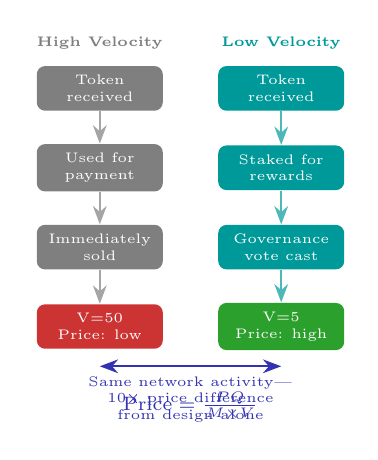
\begin{tikzpicture}[scale=0.72, every node/.style={font=\tiny},
  sbox/.style={rounded corners=3pt, minimum width=1.6cm, minimum height=0.55cm,
               align=center, font=\tiny, text=white}]
  % LEFT stack: High Velocity Token
  \node[font=\tiny\bfseries, mlgray] at (0,6.8) {High Velocity};
  \node[sbox, fill=mlgray] (h1) at (0,6.0) {Token\\received};
  \node[sbox, fill=mlgray] (h2) at (0,4.6) {Used for\\payment};
  \node[sbox, fill=mlgray] (h3) at (0,3.2) {Immediately\\sold};
  \node[sbox, fill=dfred] (h4) at (0,1.8) {V=50\\Price: low};

  \draw[->, >=Stealth, thick, mlgray!70] (h1) -- (h2);
  \draw[->, >=Stealth, thick, mlgray!70] (h2) -- (h3);
  \draw[->, >=Stealth, thick, mlgray!70] (h3) -- (h4);

  % RIGHT stack: Low Velocity Token
  \node[font=\tiny\bfseries, dfteal] at (3.2,6.8) {Low Velocity};
  \node[sbox, fill=dfteal] (l1) at (3.2,6.0) {Token\\received};
  \node[sbox, fill=dfteal] (l2) at (3.2,4.6) {Staked for\\rewards};
  \node[sbox, fill=dfteal] (l3) at (3.2,3.2) {Governance\\vote cast};
  \node[sbox, fill=mlgreen] (l4) at (3.2,1.8) {V=5\\Price: high};

  \draw[->, >=Stealth, thick, dfteal!70] (l1) -- (l2);
  \draw[->, >=Stealth, thick, dfteal!70] (l2) -- (l3);
  \draw[->, >=Stealth, thick, dfteal!70] (l3) -- (l4);

  % Bottom comparison double arrow
  \draw[<->, >=Stealth, thick, mlpurple] (h4.south) ++(0,-0.3)
    -- ++(3.2,0) node[midway, below, align=center, font=\tiny, text=mlpurple]
    {Same network activity---\\10\texttimes{} price difference\\from design alone};

  % Center formula
  \node[font=\scriptsize, mlpurple] at (1.6,0.4) {$\text{Price} = \frac{PQ}{M \times V}$};
\end{tikzpicture}
\end{column}
\end{columns}

\begin{block}{Key Insight}
Two tokens on identical networks can differ in value by a factor of ten or more---the
difference is not in what the network does, but in whether the token gives holders
a reason to keep it.
\end{block}

\bottomnote{Token velocity (how fast tokens change hands) is the single most important---and most often overlooked---driver of token value.}
\end{frame}

% ============================================================
% SLIDE 6: RISK -- What happens when the music stops?
% Visual: TikZ comic (dfred failure) RIGHT, text LEFT
% ============================================================
\begin{frame}[t]{What happens when the music stops and everyone wants out at once?}
\begin{columns}[T]
\begin{column}{0.55\textwidth}
\footnotesize
Some tokens promise to maintain a stable value---pegged to a currency. The
mechanism: if the token's price drops, holders can redeem it for newly minted
tokens of a partner asset. But what happens when everyone redeems at once?

\vspace{1mm}
\footnotesize
\begin{itemize}\compactlist
\item \textbf{Step 1 -- Peg breaks:} The stable token drops below its target price
\item \textbf{Step 2 -- Redemption rush:} Holders rush to redeem their stable
  tokens for the partner token
\item \textbf{Step 3 -- Flood of supply:} Massive new minting of the partner
  token to meet redemptions
\item \textbf{Step 4 -- Partner token crashes:} The flood of new partner tokens
  destroys their value
\item \textbf{Step 5 -- Confidence collapses:} The peg breaks further, triggering
  more redemptions
\end{itemize}

\vspace{1mm}
\scriptsize
This self-reinforcing collapse is called a death spiral (a feedback loop where each
redemption makes the next one more likely and more damaging). The algorithmic
mechanism designed to restore stability instead accelerates destruction.
\end{column}
\begin{column}{0.42\textwidth}
\centering
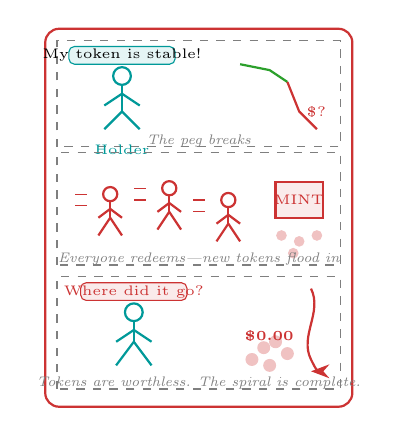
\begin{tikzpicture}[scale=0.75, every node/.style={font=\tiny}]
  % Border
  \draw[dfred, rounded corners=5pt, thick] (-0.3,-0.2) rectangle (4.9,6.2);

  % PANEL 1 (top): Holder watching price drop
  \draw[mlgray, dashed] (-0.1,4.2) rectangle (4.7,6.0);

  % Holder stick figure
  \draw[dfteal, thick] (1.0,5.4) circle (0.15);
  \draw[dfteal, thick] (1.0,5.25) -- (1.0,4.8);
  \draw[dfteal, thick] (1.0,5.1) -- (0.7,4.9);
  \draw[dfteal, thick] (1.0,5.1) -- (1.3,4.9);
  \draw[dfteal, thick] (1.0,4.8) -- (0.7,4.5);
  \draw[dfteal, thick] (1.0,4.8) -- (1.3,4.5);
  \node[below, dfteal] at (1.0,4.4) {Holder};

  % Speech bubble
  \draw[dfteal, rounded corners=2pt, fill=dfteal!10]
    (0.1,5.6) rectangle (1.9,5.9);
  \node at (1.0,5.75) {My token is stable!};

  % Price chart (dropping line)
  \draw[thick, mlgreen] (3.0,5.6) -- (3.5,5.5) -- (3.8,5.3);
  \draw[thick, dfred] (3.8,5.3) -- (4.0,4.8) -- (4.3,4.5);
  \node[dfred] at (4.3,4.8) {\$?};

  \node[mlgray, font=\tiny\itshape] at (2.3,4.3) {The peg breaks};

  % PANEL 2 (middle): Crowd rushing to redeem
  \draw[mlgray, dashed] (-0.1,2.2) rectangle (4.7,4.1);

  % Three rushing stick figures
  \draw[dfred, thick] (0.8,3.4) circle (0.12);
  \draw[dfred, thick] (0.8,3.28) -- (0.8,3.0);
  \draw[dfred, thick] (0.8,3.15) -- (0.6,3.0);
  \draw[dfred, thick] (0.8,3.15) -- (1.0,3.0);
  \draw[dfred, thick] (0.8,3.0) -- (0.6,2.7);
  \draw[dfred, thick] (0.8,3.0) -- (1.0,2.7);

  \draw[dfred, thick] (1.8,3.5) circle (0.12);
  \draw[dfred, thick] (1.8,3.38) -- (1.8,3.1);
  \draw[dfred, thick] (1.8,3.25) -- (1.6,3.1);
  \draw[dfred, thick] (1.8,3.25) -- (2.0,3.1);
  \draw[dfred, thick] (1.8,3.1) -- (1.6,2.8);
  \draw[dfred, thick] (1.8,3.1) -- (2.0,2.8);

  \draw[dfred, thick] (2.8,3.3) circle (0.12);
  \draw[dfred, thick] (2.8,3.18) -- (2.8,2.9);
  \draw[dfred, thick] (2.8,3.05) -- (2.6,2.9);
  \draw[dfred, thick] (2.8,3.05) -- (3.0,2.9);
  \draw[dfred, thick] (2.8,2.9) -- (2.6,2.6);
  \draw[dfred, thick] (2.8,2.9) -- (3.0,2.6);

  % Motion lines
  \draw[dfred] (0.4,3.4) -- (0.2,3.4);
  \draw[dfred] (0.4,3.2) -- (0.2,3.2);
  \draw[dfred] (1.4,3.5) -- (1.2,3.5);
  \draw[dfred] (1.4,3.3) -- (1.2,3.3);
  \draw[dfred] (2.4,3.3) -- (2.2,3.3);
  \draw[dfred] (2.4,3.1) -- (2.2,3.1);

  % Printer icon (MINT)
  \draw[dfred, thick, fill=dfred!10] (3.6,3.0) rectangle (4.4,3.6);
  \node[dfred, font=\tiny] at (4.0,3.3) {MINT};
  % Small token circles flying out
  \draw[dfred!30, fill=dfred!30] (3.7,2.7) circle (0.08);
  \draw[dfred!30, fill=dfred!30] (4.0,2.6) circle (0.08);
  \draw[dfred!30, fill=dfred!30] (4.3,2.7) circle (0.08);
  \draw[dfred!30, fill=dfred!30] (3.9,2.4) circle (0.08);

  \node[mlgray, font=\tiny\itshape] at (2.3,2.3) {Everyone redeems---new tokens flood in};

  % PANEL 3 (bottom): Holder with worthless tokens
  \draw[mlgray, dashed] (-0.1,0.1) rectangle (4.7,2.0);

  % Dismayed holder
  \draw[dfteal, thick] (1.2,1.4) circle (0.15);
  \draw[dfteal, thick] (1.2,1.25) -- (1.2,0.9);
  \draw[dfteal, thick] (1.2,1.1) -- (0.9,0.9);
  \draw[dfteal, thick] (1.2,1.1) -- (1.5,0.9);
  \draw[dfteal, thick] (1.2,0.9) -- (0.9,0.5);
  \draw[dfteal, thick] (1.2,0.9) -- (1.5,0.5);

  % Speech bubble
  \draw[dfred, rounded corners=2pt, fill=dfred!10]
    (0.3,1.6) rectangle (2.1,1.9);
  \node[dfred] at (1.2,1.75) {Where did it go?};

  % Pile of worthless tokens
  \draw[dfred!30, fill=dfred!30] (3.2,0.6) circle (0.1);
  \draw[dfred!30, fill=dfred!30] (3.5,0.5) circle (0.1);
  \draw[dfred!30, fill=dfred!30] (3.8,0.7) circle (0.1);
  \draw[dfred!30, fill=dfred!30] (3.4,0.8) circle (0.1);
  \draw[dfred!30, fill=dfred!30] (3.6,0.9) circle (0.1);
  \node[dfred, font=\tiny\bfseries] at (3.5,1.0) {\$0.00};

  % Downward spiral arrow
  \draw[dfred, thick, ->, >=Stealth] (4.2,1.8) .. controls (4.4,1.4) and (4.0,1.0) .. (4.2,0.6)
    .. controls (4.3,0.4) .. (4.2,0.4);

  \node[mlgray, font=\tiny\itshape] at (2.3,0.2) {Tokens are worthless. The spiral is complete.};
\end{tikzpicture}
\end{column}
\end{columns}

\begin{block}{Key Insight}
The same algorithmic mechanism designed to restore a token's value can, under stress,
create a feedback loop that destroys it---stability by algorithm is only as strong as
the faith behind it.
\end{block}

\bottomnote{Death spirals (self-reinforcing collapses where each redemption triggers the next) have destroyed billions in value and remain the central risk of algorithmic token design.}
\end{frame}

% ============================================================
% SLIDE 7: WHERE -- Why do a handful of platforms end up with everything?
% Visual: pgfplots grouped bar chart LEFT, text RIGHT
% ============================================================
\begin{frame}[t]{Why do a handful of platforms end up with almost everything?}
\begin{columns}[T]
\begin{column}{0.55\textwidth}
\centering
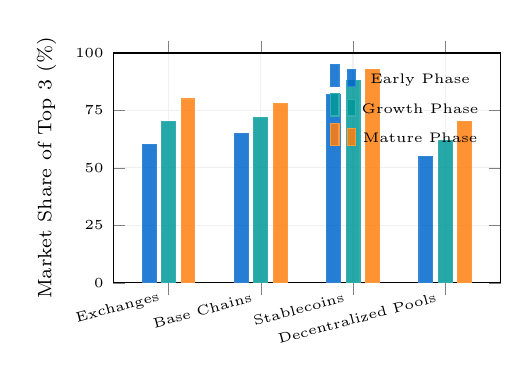
\begin{tikzpicture}
\begin{axis}[
  width=6.5cm,
  height=4.5cm,
  ybar,
  bar width=5pt,
  ymin=0, ymax=100,
  ytick={0,25,50,75,100},
  ylabel={\scriptsize Market Share of Top 3 (\%)},
  ylabel style={font=\scriptsize},
  symbolic x coords={Exchanges,Base Chains,Stablecoins,Decentralized Pools},
  xtick=data,
  xticklabel style={font=\tiny, rotate=15, anchor=east},
  yticklabel style={font=\tiny},
  legend style={font=\tiny, at={(0.98,0.98)}, anchor=north east,
    legend columns=1, draw=none, fill=none},
  grid=major,
  grid style={lightgray, thin},
  enlarge x limits=0.2,
  every axis plot/.append style={fill opacity=0.85},
]
% Critic note 2: monotonically increasing concentration trends across phases
\addplot[fill=mlblue, draw=mlblue!80] coordinates
  {(Exchanges,60) (Base Chains,65) (Stablecoins,82) (Decentralized Pools,55)};
\addplot[fill=dfteal, draw=dfteal!80] coordinates
  {(Exchanges,70) (Base Chains,72) (Stablecoins,88) (Decentralized Pools,62)};
\addplot[fill=mlorange, draw=mlorange!80] coordinates
  {(Exchanges,80) (Base Chains,78) (Stablecoins,93) (Decentralized Pools,70)};
\legend{Early Phase, Growth Phase, Mature Phase}
\end{axis}
\end{tikzpicture}
\end{column}
\begin{column}{0.42\textwidth}
\small
In platform markets, concentration is not an accident---it is the expected
outcome. When network effects mean that larger platforms offer more value per
user, growth is self-reinforcing. Even if all platforms start equal, random
early advantages compound over time.

\vspace{2mm}
\footnotesize
\begin{itemize}\compactlist
\item Proportional random growth (each platform grows by a random percentage
  of its current size) concentrates markets over time
\item Network effects accelerate this: the largest platform is also the most
  valuable per user
\item Switching costs and lock-in preserve early advantages
\item The result: a few platforms capture most of the market, across nearly
  every category
\end{itemize}
\end{column}
\end{columns}

\begin{block}{Key Insight}
Winner-take-all is not a quirk of a few markets---it is the mathematical consequence
of network effects combined with proportional growth, and it repeats across every category
of digital platform.
\end{block}

\bottomnote{Proportional random growth (Gibrat's Law) combined with network effects explains why platform markets concentrate even without deliberate monopoly strategy.}
\end{frame}

% ============================================================
% SLIDE 8: IMPACT -- Who wins and who loses?
% Visual: TikZ stakeholder map LEFT, text RIGHT
% ============================================================
\begin{frame}[t]{Who wins and who loses when one platform takes all?}
\begin{columns}[T]
\begin{column}{0.55\textwidth}
\centering
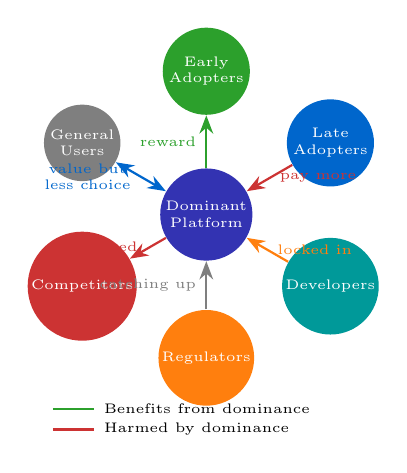
\begin{tikzpicture}[scale=0.65, every node/.style={font=\tiny},
  sat/.style={circle, minimum size=0.9cm, align=center, font=\tiny,
              text=white, inner sep=1pt}]
  % Central node
  \node[sat, fill=mlpurple, minimum size=1.1cm] (center) at (0,0)
    {Dominant\\Platform};

  % Six satellite nodes at 60-degree intervals
  \node[sat, fill=mlgreen] (early) at (90:2.8) {Early\\Adopters};
  \node[sat, fill=mlblue] (late) at (30:2.8) {Late\\Adopters};
  \node[sat, fill=dfteal] (devs) at (330:2.8) {Developers};
  \node[sat, fill=mlorange] (regs) at (270:2.8) {Regulators};
  \node[sat, fill=dfred] (comps) at (210:2.8) {Competitors};
  \node[sat, fill=mlgray] (users) at (150:2.8) {General\\Users};

  % Connecting arrows with labels
  \draw[->, >=Stealth, thick, mlgreen] (center) -- (early)
    node[midway, left, font=\tiny, text=mlgreen] {reward};
  \draw[->, >=Stealth, thick, dfred] (late) -- (center)
    node[midway, right, font=\tiny, text=dfred] {pay more};
  \draw[->, >=Stealth, thick, mlorange] (devs) -- (center)
    node[midway, right, font=\tiny, text=mlorange] {locked in};
  \draw[->, >=Stealth, thick, mlgray] (regs) -- (center)
    node[midway, left, font=\tiny, text=mlgray] {catching up};
  \draw[->, >=Stealth, thick, dfred] (center) -- (comps)
    node[midway, left, font=\tiny, text=dfred] {squeezed};
  \draw[<->, >=Stealth, thick, mlblue] (center) -- (users)
    node[midway, left, font=\tiny, text=mlblue, align=center] {value but\\less choice};

  % Legend
  \draw[thick, mlgreen] (-3.0,-3.8) -- (-2.2,-3.8)
    node[right, font=\tiny, text=black] {Benefits from dominance};
  \draw[thick, dfred] (-3.0,-4.2) -- (-2.2,-4.2)
    node[right, font=\tiny, text=black] {Harmed by dominance};
\end{tikzpicture}
\end{column}
\begin{column}{0.42\textwidth}
\small
When one platform dominates, the effects ripple through every group that
depends on it. Some benefit enormously; others pay the price. Understanding
who wins and who loses is essential for evaluating whether concentration is
healthy or harmful.

\vspace{2mm}
\footnotesize
\begin{itemize}\compactlist
\item \textbf{Early adopters:} Win big---their tokens or positions appreciate
  as the network grows
\item \textbf{Late adopters:} Pay more---fees are higher, token prices are
  inflated, and the best positions are taken
\item \textbf{Developers:} Locked in---they build for the dominant platform
  because that is where the users are, even if the platform changes terms
\item \textbf{Regulators:} Playing catch-up---the platform grows faster than
  rules can be written
\item \textbf{Competitors:} Squeezed out---network effects make it nearly
  impossible to attract users away from the dominant player
\item \textbf{General users:} Mixed---they benefit from network value (more
  counterparties, more liquidity) but lose choice and bargaining power
\end{itemize}
\end{column}
\end{columns}

\begin{block}{Key Insight}
Platform dominance is not neutral---it redistributes value from latecomers to early
movers, from competitors to the winner, and from user choice to network efficiency.
\end{block}

\bottomnote{Winner-take-all dynamics raise the same questions in digital finance that antitrust law raises in traditional markets: when does dominance become harmful?}
\end{frame}

% ============================================================
% SLIDE 9: SO WHAT -- Three questions that reveal any token's true design
% Visual: TikZ triple-balance metaphor RIGHT, text LEFT
% ============================================================
\begin{frame}[t]{Three questions that reveal any token's true design}
\begin{columns}[T]
\begin{column}{0.55\textwidth}
\small
Whether you are evaluating a new token, designing one, or deciding whether to
hold one, you can cut through the noise by asking three questions:

\vspace{2mm}
\footnotesize
\begin{enumerate}\compactlist
\item \textbf{How does it control velocity?} (Measures value capture: staking,
  burns, and governance rights slow token circulation and support price. If
  nothing slows velocity, the token's value drains away.)
\item \textbf{How does it incentivize growth?} (Measures sustainability:
  airdrops, subsidies, and fee discounts attract users---but if subsidies are
  the only reason users stay, the platform collapses when they stop.)
\item \textbf{Who controls the rules, and can they change them?} (Measures
  governance risk: centralized control is fast but fragile; decentralized
  governance is slow but resilient. The question is who has the power to change
  the token's supply, fees, or distribution.)
\end{enumerate}

\vspace{2mm}
\footnotesize
Apply these three questions to any token. A well-designed token scores well on
all three; most real tokens sacrifice one dimension for another. There is no
perfect design---only informed trade-offs.
\end{column}
\begin{column}{0.42\textwidth}
\centering
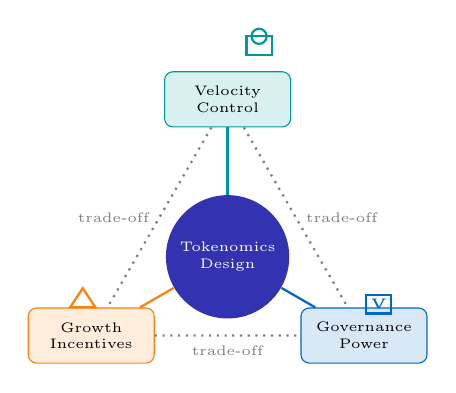
\begin{tikzpicture}[scale=0.8, every node/.style={font=\tiny}]
  % Central pivot
  \node[circle, fill=mlpurple, text=white, minimum size=0.9cm,
        font=\tiny, align=center] (pivot) at (0,0) {Tokenomics\\Design};

  % Top: Velocity Control
  \node[rounded corners=3pt, fill=dfteal!15, draw=dfteal,
        minimum width=1.6cm, minimum height=0.7cm, align=center]
    (vc) at (90:2.5) {Velocity\\Control};
  \draw[thick, dfteal] (pivot) -- (vc);
  % Lock icon
  \draw[dfteal, thick] (0.3,3.2) rectangle (0.7,3.5);
  \draw[dfteal, thick] (0.5,3.5) circle (0.12);

  % Bottom-left: Growth Incentives
  \node[rounded corners=3pt, fill=mlorange!15, draw=mlorange,
        minimum width=1.6cm, minimum height=0.7cm, align=center]
    (gi) at (210:2.5) {Growth\\Incentives};
  \draw[thick, mlorange] (pivot) -- (gi);
  % Rocket icon (simple triangle)
  \draw[mlorange, thick] (-2.5,-0.8) -- (-2.3,-0.5) -- (-2.1,-0.8) -- cycle;

  % Bottom-right: Governance Power
  \node[rounded corners=3pt, fill=mlblue!15, draw=mlblue,
        minimum width=1.6cm, minimum height=0.7cm, align=center]
    (gp) at (330:2.5) {Governance\\Power};
  \draw[thick, mlblue] (pivot) -- (gp);
  % Vote icon (ballot box)
  \draw[mlblue, thick] (2.2,-0.9) rectangle (2.6,-0.6);
  \node[mlblue, font=\tiny\bfseries] at (2.4,-0.75) {V};

  % Trade-off dotted lines
  \draw[dotted, thick, mlgray] (vc) -- (gi)
    node[midway, left, font=\tiny, text=mlgray] {trade-off};
  \draw[dotted, thick, mlgray] (vc) -- (gp)
    node[midway, right, font=\tiny, text=mlgray] {trade-off};
  \draw[dotted, thick, mlgray] (gi) -- (gp)
    node[midway, below, font=\tiny, text=mlgray] {trade-off};
\end{tikzpicture}
\end{column}
\end{columns}

\begin{block}{Key Insight}
A token that maximizes velocity control, growth incentives, and governance decentralization
simultaneously has never existed---every design is a deliberate trade-off among the three.
\end{block}

\bottomnote{Use these three questions to evaluate any token you encounter---from established platforms to the newest launches.}
\end{frame}

% ============================================================
% SLIDE 10: ACT -- Your Challenge: Design a token that doesn't collapse
% Visual: Full-width activity frame with exampleblock
% ============================================================
\begin{frame}[t]{Your Challenge: Design a token that doesn't collapse}
\small
You are launching a new platform that connects two groups of users. You must
design a token that attracts both sides, sustains itself after subsidies end,
and resists a death spiral. Use the three questions from the previous slide
as your framework.

\vspace{2mm}
\footnotesize
\begin{itemize}\compactlist
\item \textbf{Constraint 1:} Your platform has a token supply of ten million
  tokens and annual transaction volume (PQ) equivalent to one billion units.
  Choose a velocity target and compute the implied token price using MV = PQ.
  Then explain what velocity sinks (staking, burns, governance) you will use
  to hit that target.
\item \textbf{Constraint 2:} Design your bootstrap strategy. Which side of the
  market do you subsidize first? What tokens do they receive, and what happens
  when subsidies end? Describe the path to critical mass.
\item \textbf{Constraint 3:} Design the governance structure. Who can change the
  token's supply, fee rate, or staking rules? What prevents a single large holder
  from controlling the system?
\item \textbf{Deliverable:} A one-page token design with: (a) velocity target and
  mechanism, (b) bootstrap strategy with timeline, (c) governance structure,
  (d) one scenario that could trigger a death spiral and your mitigation plan.
\end{itemize}

\vspace{2mm}
\footnotesize
\textit{There is no right answer. The goal is to recognize that every design choice
helps someone and hurts someone else---and to make that trade-off explicit.}

\begin{exampleblock}{Challenge}
The test of understanding is not whether you can describe how a token works, but whether
you can design one that survives---and explain what you sacrificed to make it possible.
\end{exampleblock}

\bottomnote{Token design is applied economics---the constraints are mathematical, but the choices are human.}
\end{frame}

\end{document}
